\documentclass{article}

\usepackage[margin=1in]{geometry}
\usepackage{graphicx} % Allow image/pdf includes
\usepackage{extramarks} % Extra header marks (continued on next page)
\usepackage{amsmath} % Math enhancements
\usepackage{amsthm} % Theorem typesetting
\usepackage{amssymb} % Extended symbol collection
\usepackage{tikz} % Graphical element creation
\usetikzlibrary{automata,positioning}
\usepackage{algpseudocode} % Algorithm layout
\usepackage{enumitem} % Enumerate (lists)
\usepackage{ragged2e} % Alternative alignment
\usepackage{gensymb} % Generic symbols (degree, etc)
\usepackage{empheq} % Allow \boxed around \begin{empheq}
\usepackage{color,soul} % Highlighting
\usepackage{booktabs} % Enhanced table creation
\usepackage{multirow} % Table multi row
\usepackage{mathtools} % Math enhancements
\usepackage{bm} % Bold math
\usepackage[mathscr]{euscript} % Script variables
\usepackage{cancel} % Cancel through text
\usepackage{color,soul} % Highlighting
\usepackage{mathtools}
\usepackage{multirow}
\usepackage{mathrsfs}
\usepackage{physics}
\usepackage{gensymb}
\usepackage{siunitx}
\usepackage[cache=false]{minted}
\usepackage{subcaption}
\usepackage[cache=false]{minted}
\renewcommand{\MintedPygmentize}{/Users/logan/miniconda/bin/pygmentize}
\usepackage[scaled]{beramono}
\usepackage[T1]{fontenc}
\usepackage[]{algorithm2e}

\setlength\parindent{0pt} % No indents
\setlength{\parskip}{1em} % Paragraph skip

\newcommand{\vx}{\mathbf{x}} % x vector
\newcommand{\vy}{\mathbf{y}} % x vector

\newcommand{\pageTitle}{MEEN 644 - Homework 2}
\newcommand{\pageAuthor}{Logan Harbour}

\begin{document}

\title{\LARGE \textbf{\pageTitle} \vspace{-0.3cm}}
\author{\large \pageAuthor}
\date{\vspace{-0.6cm} \large \today \vspace{-0.4cm}}

\maketitle

\section*{Problem statement}

Consider one-dimensional heat conduction in a cylindrical copper rod of length 1.0 m long. The diameter of the rod is 0.05 m. The left end of the rod is held at 100 $^\circ$C and the ambient temperature is 25 $^\circ$C. Heat is transported from the surface of the rod and the right end of the rod through natural convection to the ambient. The natural convection heat transfer coefficient is 0.5 W/m$^2~^\circ$C. Write a finite volume code to predict temperature distribution as a function of length. Use TDMA to solve a set of discretization equations. Make calculations using ITMAX: 6, 11, 21, 41, and 81 nodes. Plot your results.

\section*{Preliminaries}

\subsection*{One-dimensional heat conduction}

With one-dimensional heat conduction with convection and constant material properties, we have the ODE
\begin{equation}
	\begin{cases}
		\dv{^2T}{x^2} + \frac{h}{kd} (T - T_\infty) = 0\,,\\
		T(0) = T_0\,,\\
		\dv{T}{x} \big|_{x = L} = - \frac{h}{k} (T - T_\infty)\,,
	\end{cases}
\end{equation}
where
\begin{align*}
	k & \equiv 400~\text{W/m}~^\circ\text{C}\,, & h & \equiv 0.5~\text{W/m}^2~^\circ\text{C}\,, & d & \equiv 0.05~\text{m}\,,\\
	L & \equiv 1.0~\text{m}\,, & T_0 & \equiv 100~^\circ\text{C}\,, & T_\infty & \equiv 25~^\circ\text{C}\,.\\
\end{align*}
We then make the substitutions $\theta(x) = T(x) - T_\infty$ and $m = 4h/kd$ to obtain the simplification
\begin{equation}
	\begin{cases}
		\dv{^2\theta}{x^2} + m \theta = 0\,,\\
		\theta(0) = T_0 - T_\infty\,,\\
		\dv{\theta}{x} \big|_{x = L} = - \frac{h}{k} \theta\,.
	\end{cases}
	\end{equation}

\subsection*{Grid generation}

We discretize the region on $x = [0, L]$ by $N$ (also defined as ITMAX) nodes and $N$ control volumes, as follows in Figure \ref{fig:CVs} with $\Delta x = L / (N - 1)$.

\begin{figure}[H]
	\centering
	\begin{subfigure}[t]{0.32\textwidth}
		\centering
		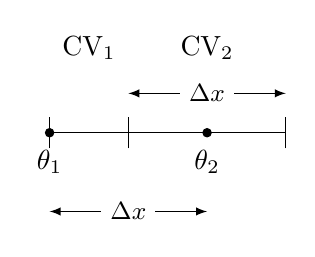
\begin{tikzpicture}[scale=2]
			\tikzset{dimen/.style={<->,>=latex,thin,every rectangle node/.style={fill=white,midway,font=\small}}}

			\draw (0,0) -- (1.5, 0);

			\foreach \i in {0, 0.5, 1.5}
				\draw (\i, -0.1) -- (\i, 0.1);

			\foreach \i in {0, 1}
				\filldraw (\i, 0) circle (0.75pt);

			\node[below] at (0, -0.05) {$\theta_1$};
			\node[below] at (1, -0.05) {$\theta_2$};
			\node[above] at (0.25, 0.4) {CV$_1$};
			\node[above] at (1, 0.4) {CV$_2$};

			\draw [dimen] (0.5, 0.25) -- (1.5, 0.25) node {$\Delta x$};
			\draw [dimen] (0.0, -0.5) -- (1.0, -0.5) node {$\Delta x$};
		\end{tikzpicture}
		\caption{Left CV}
	\end{subfigure}
	\hfill
	\begin{subfigure}[t]{0.32\textwidth}
		\centering
		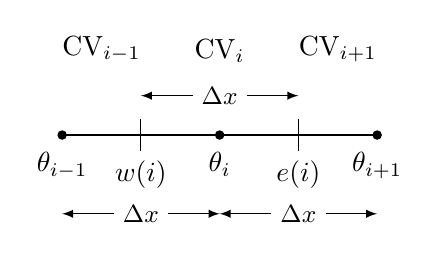
\begin{tikzpicture}[scale=2]
			\tikzset{dimen/.style={<->,>=latex,thin,every rectangle node/.style={fill=white,midway,font=\small}}}

			\draw (0,0) -- (2,0);

			\foreach \i in {0.5, 1.5}
				\draw (\i, -0.1) -- (\i, 0.1);

			\foreach \i in {0, 1, 2}
			\filldraw (\i, 0) circle (0.75pt);

			\node[below] at (0, -0.05) {$\theta_{i-1}$};
			\node[below] at (1, -0.05) {$\theta_i$};
			\node[below] at (2, -0.05) {$\theta_{i+1}$};
			\node[below] at (1.5, -0.1) {$e(i)$};
			\node[below] at (0.5, -0.1) {$w(i)$};
			\node[above] at (1.0, 0.4) {CV$_i$};
			\node[above] at (0.25, 0.4) {CV$_{i-1}$};
			\node[above] at (1.75, 0.4) {CV$_{i+1}$};

			\draw [dimen] (0.5, 0.25) -- (1.5, 0.25) node {$\Delta x$};
			\draw [dimen] (0, -0.5) -- (1.0, -0.5) node {$\Delta x$};
			\draw [dimen] (1, -0.5) -- (2.0, -0.5) node {$\Delta x$};
		\end{tikzpicture}
		\caption{Interior CV ($1 < i < N$)}
	\end{subfigure}
	\hfill
	\begin{subfigure}[t]{0.32\textwidth}
		\centering
		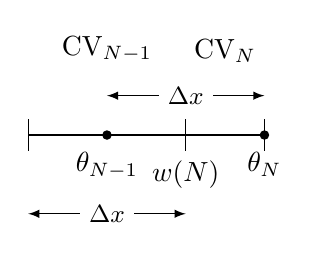
\begin{tikzpicture}[scale=2]
			\tikzset{dimen/.style={<->,>=latex,thin,every rectangle node/.style={fill=white,midway,font=\small}}}

			\draw (0,0) -- (1.5,0);

			\foreach \i in {0, 1, 1.5}
				\draw (\i, -0.1) -- (\i, 0.1);

			\foreach \i in {0.5, 1.5}
				\filldraw (\i, 0) circle (0.75pt);

			\node[below] at (0.5, -0.05) {$\theta_{N-1}$};
			\node[below] at (1.5, -0.05) {$\theta_N$};
			\node[above] at (1.25, 0.4) {CV$_N$};
			\node[above] at (0.5, 0.4) {CV$_{N-1}$};
			\node[below] at (1.0, -0.1) {$w(N)$};

			\draw [dimen] (0.5, 0.25) -- (1.5, 0.25) node {$\Delta x$};
			\draw [dimen] (0.0, -0.5) -- (1.0, -0.5) node {$\Delta x$};
		\end{tikzpicture}
		\caption{Right CV}
	\end{subfigure}
	\caption{The control volumes defined for discretization of the problem.}
	\label{fig:CVs}
\end{figure}

\subsection*{Equation discretization}

\subsubsection*{Internal control volume equation}

We start with the integration over an interior control volume, as
\[
	\int_{\text{CV}_i} \left[ -\dv{^2\theta}{x^2} + m \theta \right] dx = 0\,, \quad 1 < i < N\,,
\]
in which we know that the material properties are independent and we assume $\theta_i$ to be constant over the cell for the second term to obtain
\[
	- \left( \dv{\theta}{x}\Big|_{e(i)} - \dv{\theta}{x}\Big|_{w(i)} \right) + m \Delta x \theta_i = 0\,, \quad 1 < i < N\,.
\]
Use the two node formulation for the derivative terms and simplify as
\begin{align*}
	- \left( \frac{\theta_{i+1} - \theta_i}{\Delta x} - \frac{\theta_i - \theta_{i - 1}}{\Delta x} \right) + m \Delta x \theta_i & = 0 \,, \quad 1 < i < N\,, \\
	- \frac{1}{\Delta x} \theta_{i-1} + \left(m \Delta x + \frac{2}{\Delta x}\right) \theta_i - \frac{1}{\Delta x} \theta_{i+1} & = 0\,, \quad 1 < i < N\,.
\end{align*}
Take note that at the $i = 2$ equation, $\theta_1$ is known therefore we have
\begin{align}
	\Aboxed{\left(m \Delta x + \frac{2}{\Delta x}\right) \theta_2 - \frac{1}{\Delta x} \theta_3 & = \frac{T_0 - T_\infty}{\Delta x}\,,}\\
	\Aboxed{- \frac{1}{\Delta x} \theta_{i-1} + \left(m \Delta x + \frac{2}{\Delta x}\right) \theta_i - \frac{1}{\Delta x} \theta_{i+1} & = 0\,, \quad 2 < i < N\,.}
\end{align}

\subsubsection*{Right control volume equation}

We start with the integration over the right control volume, CV$_N$, as
\[
	\int_{\text{CV}_N} \left[ -\dv{^2\theta}{x^2} + m \theta \right] dx = 0\,,
\]
in which for the second term we will assume $\theta_N$ to be constant over CV$_N$ to obtain
\[
	- \left( \dv{\theta}{x}\Big|_{x = L} - \dv{\theta}{x}\Big|_{w(N)} \right) + \frac{1}{2} m \Delta x \theta_N = 0\,.
\]
Use the two node formulation for the derivative term at $w(N)$ and the right boundary condition for the derivative term at $x = L$ m to obtain
\begin{align}
	\frac{h}{k} \theta_N + \frac{\theta_N - \theta_{N-1}}{\Delta x} + \frac{1}{2} m \Delta x \theta_N & = 0\,,\nonumber\\
	\Aboxed{- \frac{1}{\Delta x} \theta_{N-1} + \left(\frac{1}{2} m \Delta x + \frac{h}{k} + \frac{1}{\Delta x}\right) \theta_N & = 0\,.}
\end{align}

\subsection*{TDMA}

The system we are solving is of the form
\renewcommand*{\arraystretch}{1.3}
\[
	\begin{bmatrix}
		b_1 & c _1 & & & 0 \\
		a_2 & b_2 & c_2 \\
		& a_3 & b_3 & \ddots & \\
		& & \ddots & \ddots & c_{n - 1} \\
		0 & & & a_n & b_n
	\end{bmatrix}
	\begin{bmatrix}
		x_1 \\
		x_2 \\
		x_3 \\
		\vdots \\
		x_n
	\end{bmatrix}
	=
	\begin{bmatrix}
		d_1 \\
		d_2 \\
		d_3 \\
		\vdots \\
		d_n
	\end{bmatrix}\,.
\]
We will solve this system using the tridiagonal matrix algorithm (TDMA) given the fact that our system is positive definite. With our matrix in the form above, the algorithm follows in Algorithm \ref{alg:tdma}. Note that for the algorithm below, we are solving the solution vector $\vec{x}$ in-place with the vector $\vec{d}$. This algorithm is in the member function \texttt{solveTDMA()} in the \texttt{TriDiagonal} class, which stores the left hand side system in the vectors $\vec{a}, \vec{b}$, and $\vec{c}$.

\begin{algorithm}[H]
	\For{$i = 2, 3, \ldots, n$}{
		$w = a_i / b_{i - 1}$\;
		$b_i = b_i - w c_{i - 1}$\;
		$d_i = d_i - w d_{i - 1}$\;
	}
	$d_n = d_n / b_n$\;
	\For{$i = n - 1, n - 2, \ldots, 1$}{
		$d_i = d_i - c_i d_{i+1}$\;
		$d_i = d_i / b_i$\;
	}
	\caption{The tridiagonal matrix algorithm (TDMA).}
	\label{alg:tdma}
\end{algorithm}

\section*{Results}

The plotted results as requested follow below in Figure \ref{fig:results}. In addition, the solution for ITMAX = 6 is tabulated in Table \ref{table:results}.

\begin{figure}[H]
	\centering
	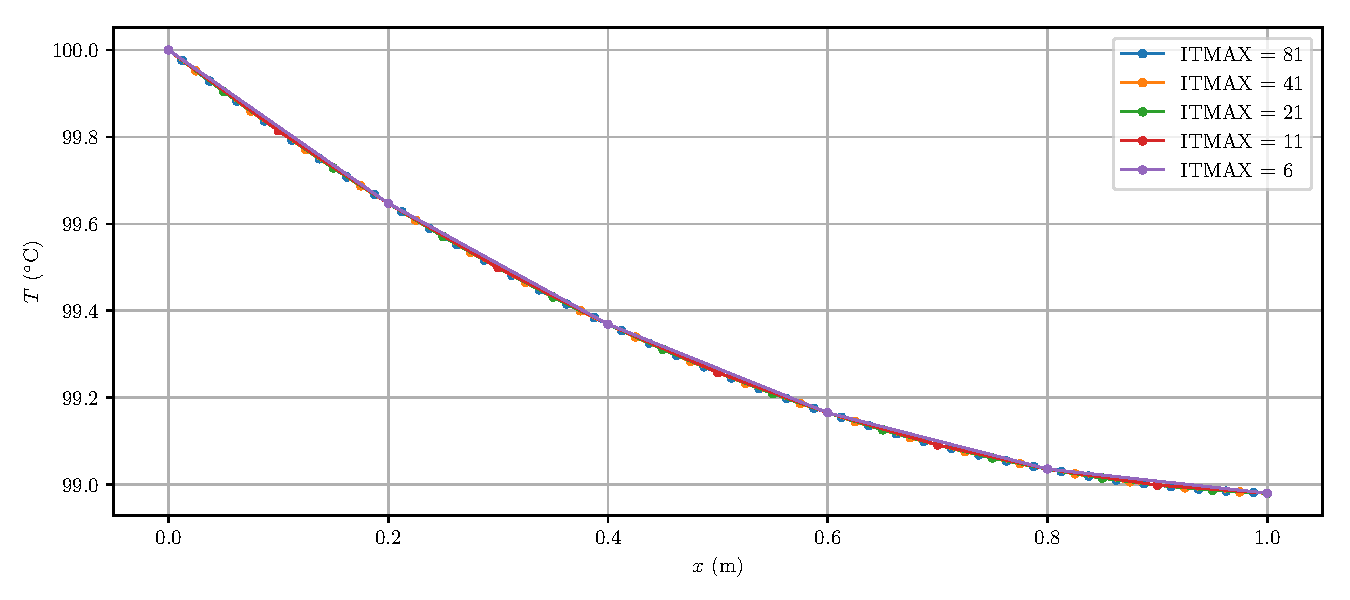
\includegraphics[width=\linewidth]{../python/result}
	\caption{The plotted solution.}
	\label{fig:results}
\end{figure}

\def\arraystretch{1.3}
\begin{table}[H]
	\small
	\centering
	\caption{The solution for ITMAX = 6.}
	\vspace{0.2cm}
	\begin{tabular}{c|S[table-format=2.5,group-digits=false]|S[table-format=3.5,group-digits=false]}
		\hline
		$x$              & {$\theta$}         & {$T$}             \\
		\scriptsize{(m)} & {\scriptsize{($^\circ$C)}} & {\scriptsize{($^\circ$C)}} \\ \hline
		0.0              & 75.00000           & 100.00000 \\
		0.2              & 73.68060           &  98.68060 \\
		0.4              & 72.65593           &  97.65593 \\
		0.6              & 71.92188           &  96.92188 \\
		0.8              & 71.47552           &  96.47552 \\
		1.0              & 71.31506           &  96.31506 \\
	\end{tabular}
	\label{table:results}
\end{table}

\section*{Code listing}

\subsection*{Makefile}

\inputminted[fontsize=\small]{Makefile}{../cpp/Makefile}

\subsection*{hwk2.cpp}

\inputminted[fontsize=\small]{c++}{../cpp/hwk2.cpp}

\subsection*{TriDiagonal.h}

\inputminted[fontsize=\small]{c++}{../cpp/TriDiagonal.h}

\end{document}
